\section{Programming Expositions}
\begin{topics}
All previous sections.
\end{topics}
\subsection{Newton Interpolation}
For a given sequence of numbers $\{a_0,\ldots,a_{n-1}\}$, we define $\Delta ^{k}$ inductively as follows
\begin{itemize}
	\item $\Delta ^{0}=\{a_0,\ldots,a_{n-1}\}$
	\item If $\Delta ^{i}=\{b_0,b_1,\ldots,b_{n-i-2},b_{n-i-1}\}$ then $\Delta ^{i+1}=\{b_1-b_0,\ldots,b_{n-i-1}-b_{n-i-2}\}$; i.e., difference of succesive terms gives the next sequence. Also, we treat $\Delta ^{k}$ as an array with $i$\textsuperscript{th} index as $\Delta ^{k}[i]$.
\end{itemize}
Notice, that number of terms reduces by 1 after each iteration. Hence $\Delta ^{n-1}$ has only 1 term and we stop.

Now, using these $\Delta ^{i}$'s, we can constuct a polynomial $f$ such that $f(i)=a_i$ for $i=\{0,1,\ldots,n-1\}$. This process is called \emph{interpolation} and the formula for $f$ is given below.
\begin{equation}
	f(x)=\sum _{k=0}^{n-1}{\binom {x}{k}}\,\Delta ^{k}[0]=\sum _{k=0}^{n-1}\frac{(x)_k}{k!}\,\Delta ^{k}[0]%\sum _{k=0}^{\infty }{\frac {\Delta ^{k}[a]}{k!}}\,(x-a)_{k}=
	\quad\text{ where $(x)_0 = 1$ and $(x)_k=x(x-1)\cdots(x-(k-1))$}
\end{equation}
An example from \href{https://en.wikipedia.org/wiki/Finite_difference#Newton's_series}{wikipedia},
\vspace{-1em}\begin{equation}
	{{
	\begin{matrix}{
	\begin{array}{c|ccc} x&f=\Delta ^{0}&\Delta ^{1}&\Delta ^{2}\\\hline 0&{\underline {2}}&&\\
	&&{\underline {0}}&\\
	1&2&&{\underline {2}}\\
	&&2&\\
	2&4&&
	\end{array}}
	&\quad {
	\begin{aligned}
	f(x)&=\Delta ^{0}\cdot {\dfrac {(x)_{0}}{0!}}+\Delta ^{1}\cdot {\dfrac {(x)_{1}}{1!}}+\Delta ^{2}\cdot {\dfrac {(x)_{2}}{2!}}\quad\\\\
	&=2\cdot 1+0\cdot {\dfrac {x}{1}}+2\cdot {\dfrac {(x)(x-1)}{2}}\\\\
	&=2+(x)(x-1)
	\end{aligned}}\end{matrix}}}\vspace{-0.5em}
\end{equation}
\textbf{Problem Statement:}\\
For a given sequence $\{a_0,\ldots,a_{n-1}\}$, find its interpolated polynomial and predict the next term $a_{n}=f(n)$.
\begin{testcases}
	{$t$ \hfill(number of test cases, an integer)\\$n_i\quad a_{0}\ a_1\ \ldots\ a_{n_i-1}$ \hfill($n_i+1$ space seperated integers for each testcase)}
	{$f(n_i)$, followed by expansion of $f(x)\displaystyle\sum _{k=0}^{n-1}\frac{x_k}{k!}\,\Delta ^{k}[0]$, ignoring $\Delta ^{i}[0]=0$ terms and $\Delta ^{i}[0]=\pm1$ coefficients.}
	{$1 \leq n_i \leq 20$, $-1000 \leq a_i \leq 1000$}
	{4\\3\quad2 2 4\\4\quad1 2 3 4\\7\quad3 1 4 1 5 9 2\\9\quad1 2 4 8 16 31 57 99 163}
	{8\quad2(x)\_{0}/0! + 2(x)\_{2}/2!\\5\quad(x)\_{0}/0! + (x)\_{1}/1!\\45\quad3(x)\_{0}/0! - 2(x)\_{1}/1! + 5(x)\_{2}/2! - 11(x)\_{3}/3! + 24(x)\_{4}/4! - 44(x)\_{5}/5! + 60(x)\_{6}/6!\\256\quad(x)\_{0}/0! + (x)\_{1}/1! + (x)\_{2}/2! + (x)\_{3}/3! + (x)\_{4}/4!}
	{https://github.com/paramrathour/CS-101/tree/main/Starter Codes/Newton Interpolation.cpp}
\end{testcases}
\begin{funvideo}
	\href{https://youtu.be/4AuV93LOPcE}{Why don't they teach Newton's calculus of `What comes next?' -- Mathologer}
\end{funvideo}
\KOMAoptions{paper=A3}
\recalctypearea
\subsection{Vigen\'ere Cipher}
Vigen\'ere Cipher is an cryptographic technique used for encryption and decryption of alphabetic texts. The process is done letter-by-letter.
\subsubsection*{Encryption}
\begin{itemize}
	\item Generate a message (also called as a plaintext) and an empty ciphertext.
	\item Select a key; i.e., a string of alphabets. Keep repeating the key until it is as long as message.
	\item Iterate through the message and key simulataneously, to get current message alphabet and key alphabet.
	\item Now from the table \ref{fig:vignerecipher}, insert into ciphertext the alphabet corresponding to message alphabet as row and key alphabet as column.
\end{itemize}
\subsubsection*{Decryption}
\begin{itemize}
	\item In this case, key and ciphertext are known.
	\item Iterate through the key and ciphertext simulataneously, to get current key letter and ciphertext letter.
	\item Now from the table \ref{fig:vignerecipher}, find the ciphertext letter in the column corresponding to the current key letter. The row of ciphertext letter gives plaintext letter.
\end{itemize}
\begin{note}
	The encryption and decryption hinges on the fact that the key is kept secret and known only to people encrypting and decrypting the messages.\\
	With the knowledge of key, decryption is ``easy'' but without key it is ``hard''.
\end{note}
\begin{figure}[H]
	\centering
	\includegraphics[width = 0.5\linewidth]{Vigenère Square.pdf}
	\caption{The Vigenere square (\href{https://commons.wikimedia.org/wiki/File:Vigenère_square_shading.svg}{Image} by \href{https://en.wikipedia.org/wiki/User:Matt_Crypto}{Matt Crypto}, Public domain, via Wikimedia Commons)}
	\label{fig:vignerecipher}
\end{figure}
\textbf{Problem Statement:}\\
Implement encryption and decryption function as stated above:
\begin{testcases}
	{$t$ \hfill(number of test cases, an integer)\\$k_i\ p_i$\hfill(size of key and plaintext for each testcase)\\
	$K_{0}\ldots K_{k_i}$\hfill(key)\\
	$P_{0}\ldots P_{p_i}$\hfill(plaintext)}
	{Ciphertext\hfill(Verify decryption manually for decrypting the generated ciphertext and comparing with plaintext)}
	{$1 \leq k_i, p_i \leq 1000$, $K_i, P_i$ are CAPITAL LETTERS.}
	% {6\\
	% 5 12\\
	% LEMON\\
	% ATTACKATDAWN\\
	% 16 39\\
	% LEOPOLDKRONECKER\\
	% GODMADETHEINTEGERSALLELSEISTHEWORKOFMAN\\
	% 17 136\\
	% STUARTMILNERBARRY\\
	% IDONOTIMAGINETHATANYWARSINCECLASSICALTIMESIFEVERHASBEENFOUGHTINWHICHONESIDEREADCONSISTENTLYTHEMAINMILITARYANDNAVALINTELLIGENCEOFTHEOTHER\\
	% 15 201\\
	% BERTRANDRUSSELL\\
	% MATHEMATICSPOSSESSESNOTONLYTRUTHBUTASUPREMEBEAUTYCOLDANDAUSTERELIKETHATOFSCULPTUREWITHOUTTHEGORGEOUSTRAPPINGSOFPAINTINGORMUSICYETSUBLIMELYPUREANDCAPAB
	% LEOFASTERNPERFECTIONSUCHASONLYTHEGREATESTARTCANSHOW\\
	% 15 382\\
	% BERTRANDRUSSELL\\
	% IOUGHTTOCALLMYSELFANAGNOSTICBUTFORALLPRACTICALPURPOSESIAMANATHEISTIDONOTTHINKTHEEXISTENCEOFTHECHRISTIANGODANYMOREPROBABLETHANTHEEXISTENCEOFTHEGODSOFOLY
	% MPUSORVALHALLATOTAKEANOTHERILLUSTRATIONNOBODYCANPROVETHATTHEREISNOTBETWEENTHEEARTHANDMARSACHINATEAPOTREVOLVINGINANELLIPTICALORBITBUTNOBODYTHINKSTHISSUF
	% FICIENTLYLIKELYTOBETAKENINTOACCOUNTINPRACTICEITHINKTHECHRISTIANGODJUSTASUNLIKELY\\
	% 9 389\\
	% CARLSAGAN\\
	% THEEARTHISAVERYSMALLSTAGEINAVASTCOSMICARENATHINKOFTHEENDLESSCRUELTIESVISITEDBYTHEINHABITANTSOFONECORNEROFTHISPIXELONTHESCARCELYDISTINGUISHABLEINHABITANTSOFSO
	% MEOTHERCORNERHOWFREQUENTTHEIRMISUNDERSTANDINGSHOWEAGERTHEYARETOKILLONEANOTHERHOWFERVENTTHEIRHATREDSTHINKOFTHERIVERSOFBLOODSPILLEDBYALLTHOSEGENERALSAN
	% DEMPERORSSOTHATINGLORYANDTRIUMPHTHEYCOULDBECOMETHEMOMENTARYMASTERSOFAFRACTIONOFADOT}
	% {LXFOPVEFRNHR\\\\
	% RSRBOOHDYSVRVOKVCWOAZPOCVWFXJOAFCOCUALQ\\\\
	% AWINFMUULTMEFTYRRSGSWRKEQYPITMAJJGUTFTZFQATSIMFRYRQTXYNWHGOSGMEXHZTFGGYSZWQZPNHTPNJZQLXHTCRFPPZEZOMZCGLTLYRGPVLIECJNKVJDBAEEVQWQGLVPTYVP\\\\
	% NEKAVMNWZWKHSDDFWJXJNBWFHDQXCFULSNKAFXGLWEIMPBYKRTOYGRHVSYDEFVVEZKRWYULGJDNVPGMLRRZZNZGYEEIIXHIGRRLMLJEAAJRXLFFCDZHLARRZSQLLZCLHKMMTPTXFPPILRRDEXUST
	% LMMIFYRSGHIHHWVQPDXZHESHFYUKGRWJULVZIENWVMLSVENBRJAFW\\\\
	% JSLZYTGRTUDDQJDFPWTEATQFMLAGMFUJFKRLYSIUULMNLMTLKGOFHJCSEEYLULVBJTVGFHGLXSTOOKAVEKLJNWFGPZGXYXTHELJNASRRZEEERDOEHGLGTEMWFXYTETUHVRAKXPYDIFYKHRJFXKGJZ
	% WZQGNJOEYRFZSPWLUSKTBENQFNZWVTWMYJMIAGLFHFGFZOZGRGGRBYVNZSXESFVVBJNBWSYLOIPYULVXRRGKRHVEECDBGYBEAGHRJGLVPGPPMBEGVQRHWDPTAUMTTCOEEZNTMXYZCSURKHVQB\\MLZMDDVJWBTIRQKFQDMVPMCKHSEGDBYFAREZBGTHLNGLEJJSGETDIZMYIANKBWULCTTXZTEGBGAOKLEDFOPZDVLL\\\\
	% VHVPSRZHVUAMPJYYMNNLJESGKIACVRDLCUSZKCRCWNGTUKNBZXTNERPDCPKSIRHGLKTWSBIFKTVOTYZHRKNYLTIZAAVSFQGNKCBTNVCGFZHVUPZIWLUNGJEJNSRIEYADZDLITGHKSYLTLKIAJASTLAT\\TFQFJZEEUTUGRTZJNKRUQWWCWQAEAVTYPARSIFWNUPJSZAAFIERKHUWRCGVCLHKYNTEKZCIRLBPERYGTNEEJONQWRBEAVTYPARNAGTEUDLHONXQFKSWROVRTSFQTLUOQUPZWDEJBLCLCEZOYET\\GNVCSLYAAFEDAWRURFUOKSSTONTNOIJSNJTEKUDAZTNELEOLWVBKCBOEKSWMUMRPTRCQMGSGGRJZXALRNETZZFOLAQQT}
	{6\\
	5 12\\
	LEMON\\
	ATTACKATDAWN\\\\
	16 39\\
	LEOPOLDKRONECKER\\
	GODMADETHEINTEGERSALLELSEISTHEWORKOFMAN\\\\
	17 136\\
	STUARTMILNERBARRY\\
	IDONOTIMAGINETHATANYWARSINCECLASSICALTIMESIFEVERHASBEENFOUGHTINWHICHONESIDEREADCONSISTENTLYTHEMAINMILITARYAND\\NAVALINTELLIGENCEOFTHEOTHER\\\\
	15 201\\
	BERTRANDRUSSELL\\
	MATHEMATICSPOSSESSESNOTONLYTRUTHBUTASUPREMEBEAUTYCOLDANDAUSTERELIKETHATOFSCULPTUREWITHOUTTHEGORGEOUSTRA\\PPINGSOFPAINTINGORMUSICYETSUBLIMELYPUREANDCAPABLEOFASTERNPERFECTIONSUCHASONLYTHEGREATESTARTCANSHOW\\\\
	15 382\\
	BERTRANDRUSSELL\\
	IOUGHTTOCALLMYSELFANAGNOSTICBUTFORALLPRACTICALPURPOSESIAMANATHEISTIDONOTTHINKTHEEXISTENCEOFTHECHRISTIANGODA\\NYMOREPROBABLETHANTHEEXISTENCEOFTHEGODSOFOLYMPUSORVALHALLATOTAKEANOTHERILLUSTRATIONNOBODYCANPROVETHATTH\\EREISNOTBETWEENTHEEARTHANDMARSACHINATEAPOTREVOLVINGINANELLIPTICALORBITBUTNOBODYTHINKSTHISSUFFICIENTLYLIKELYTO\\BETAKENINTOACCOUNTINPRACTICEITHINKTHECHRISTIANGODJUSTASUNLIKELY\\\\
	9 389\\
	CARLSAGAN\\
	THEEARTHISAVERYSMALLSTAGEINAVASTCOSMICARENATHINKOFTHEENDLESSCRUELTIESVISITEDBYTHEINHABITANTSOFONECORNEROFTHIS\\PIXELONTHESCARCELYDISTINGUISHABLEINHABITANTSOFSOMEOTHERCORNERHOWFREQUENTTHEIRMISUNDERSTANDINGSHOWEAGERTHEY\\ARETOKILLONEANOTHERHOWFERVENTTHEIRHATREDSTHINKOFTHERIVERSOFBLOODSPILLEDBYALLTHOSEGENERALSANDEMPERORSSOTHA\\TINGLORYANDTRIUMPHTHEYCOULDBECOMETHEMOMENTARYMASTERSOFAFRACTIONOFADOT}
	{LXFOPVEFRNHR\\\\
	RSRBOOHDYSVRVOKVCWOAZPOCVWFXJOAFCOCUALQ\\\\
	AWINFMUULTMEFTYRRSGSWRKEQYPITMAJJGUTFTZFQATSIMFRYRQTXYNWHGOSGMEXHZTFGGYSZWQZPNHTPNJZQLXHTCRFPPZEZOMZCG\\LTLYRGPVLIECJNKVJDBAEEVQWQGLVPTYVP\\\\
	NEKAVMNWZWKHSDDFWJXJNBWFHDQXCFULSNKAFXGLWEIMPBYKRTOYGRHVSYDEFVVEZKRWYULGJDNVPGMLRRZZNZGYEEIIXHIGRRLMLJ\\EAAJRXLFFCDZHLARRZSQLLZCLHKMMTPTXFPPILRRDEXUSTLMMIFYRSGHIHHWVQPDXZHESHFYUKGRWJULVZIENWVMLSVENBRJAFW\\\\
	JSLZYTGRTUDDQJDFPWTEATQFMLAGMFUJFKRLYSIUULMNLMTLKGOFHJCSEEYLULVBJTVGFHGLXSTOOKAVEKLJNWFGPZGXYXTHELJNASRR\\ZEEERDOEHGLGTEMWFXYTETUHVRAKXPYDIFYKHRJFXKGJZWZQGNJOEYRFZSPWLUSKTBENQFNZWVTWMYJMIAGLFHFGFZOZGRGGRBYVN\\ZSXESFVVBJNBWSYLOIPYULVXRRGKRHVEECDBGYBEAGHRJGLVPGPPMBEGVQRHWDPTAUMTTCOEEZNTMXYZCSURKHVQBMLZMDDVJWBTIR\\QKFQDMVPMCKHSEGDBYFAREZBGTHLNGLEJJSGETDIZMYIANKBWULCTTXZTEGBGAOKLEDFOPZDVLL\\\\
	VHVPSRZHVUAMPJYYMNNLJESGKIACVRDLCUSZKCRCWNGTUKNBZXTNERPDCPKSIRHGLKTWSBIFKTVOTYZHRKNYLTIZAAVSFQGNKCBTNVCG\\FZHVUPZIWLUNGJEJNSRIEYADZDLITGHKSYLTLKIAJASTLATTFQFJZEEUTUGRTZJNKRUQWWCWQAEAVTYPARSIFWNUPJSZAAFIERKHUWRCGV\\CLHKYNTEKZCIRLBPERYGTNEEJONQWRBEAVTYPARNAGTEUDLHONXQFKSWROVRTSFQTLUOQUPZWDEJBLCLCEZOYETGNVCSLYAAFEDAWR\\URFUOKSSTONTNOIJSNJTEKUDAZTNELEOLWVBKCBOEKSWMUMRPTRCQMGSGGRJZXALRNETZZFOLAQQT}
	{https://github.com/paramrathour/CS-101/tree/main/Starter Codes/Newton Interpolation.cpp}
\end{testcases}
\begin{funvideo}
	\href{https://youtu.be/T59hl2nlrT0}{Cracking the Cipher Challenge | Simon Singh | GOTO 2016}\\
	\href{https://youtube.com/playlist?list=PLDzQHsXy3284WoBU0pj3x0Oq9n69uOIjy}{The Science of Secrecy -- Simon Singh}
\end{funvideo}
\subsubsection*{A Challenge}
Can you decrypt this ciphertext? Key is not provided :)
\begin{tcolorbox}[breakable, enhanced, sharpish corners]
KHGPYVJLCJAPEPYYOYUGCWJGNVOIUOPBGDOTZCMXGDCVGCZIPOVDIQXGZCZYPLUHDGYGCQPHWCBVHUUSHPWQENKYXOTTUMOUBWJK\\OPMVKMLHGFGYHGFGYCLEUACLEUAWQENKHVZTVPGSVOYJOEVPGBGKBKCVYUEUUOYIYVABCDKKCQDCANJOEVJACJVJVYNPYHYTOCOIQB\\NJSPRNJSUPMUYOLNJSPNSQEVOCPUVOCUSUIUFDJPMVRKZWJSEHHGBAOYUNQUYYYTZYVRCAVKVNIICBFHLGIQBNGVNPHIWGABCDCTUPT\\WZNJKRWYPCVVZCVNSCMOVOUVXQOYQBEOYUDTHNGNKADKWOFBGNGMYEKVLXVRTVOIRCZOPBQVZCXFPMCFGKBKWCUXKCJVONNPABC\\FGPNQYMOCOSPAIOIQDHHSTTQJKVDUUSVOCPUKUAJONSHGFGYWJKPNYJONSHGFGYWJKPNYGFGYMKXELBGGCZHKXGHFYKAZNJOUHGGM\\QBFFXVRYGZJPMJKPKMQEVVZVRGJUURFYUYOTIOVXQAIWBLPGOIEVONNPAVGZTLWKYWZDKWOFMVOCSCPQVOYOLNPHFKPKBGQGAMVYD\\LUNKYFYTGJHNCCKJELYMLCURQBFFFGZNQZRLXJSODBGXKOUFDJLWJKPJYCXFFIWIQBBCFGAIUDQWBKW
% WKNHRWATHHAIXRFUVOTQDSNGKBJOFIESALFLVLIPLEKTJEJMBOUQRRLGZQZOAIRDHOSGDJLCJITTNEJGTSDIXOBGCMTMNOVQIMIUPLQVHSGNRZVPBOWYULHWZBKJHWKACEMXQWNTVDGIGLVFSMPPHUCFOQUTEETIGRFARWRJHBKDVSKYHDIYFRNAZPQPGSCGSPPLKLKAVCVHVRBRVSTCVVMOLBJIAKPMIDICQNRJPAKSOEURVSTNKLQEOQEAAIIWVOTXRQCYVZUEGLRRPSMFERYTKITELSLRSVMCQJKGAPCTNQRLXETNKDNRLVUTBJRJZVJEHWFCAVQHRSIAVOTNUDRGKQVJVQDWVOEYIHACAMFTUVFSURBMXQPQVNCNQMJYJOEBLPYPKQUHBYCBBDIUYHGVVWMHVQZLHYNSRZLHPZOWUEKUOCJNKLLMPVIHRPCLSFFLFKYPNMJEYPECJOSWKDLILMXEEWZLQOIYZDQPPVGAYARWGDIYVDKGJWWLQRKISOQBLVFCULUOHXFDHRFWDVFFYIYEEFLRBYUIXUHKTUACBYCBBDCYSUCEPWWSWMDKMCUYDOGPNBJEZFCGBNBHGKCILBUTBFVYZKXSHUUJHBCSVGBHCUFCVKMWSLXEFXFNDOEBLPUJLVKHNHKFSMIUQFCCULAOHCFSVKWYWRQVVXJIZ
\end{tcolorbox}
\KOMAoptions{paper=A4}
\recalctypearea
\KOMAoptions{paper=A3}
\recalctypearea
\subsection{Linear Feedback Shift Register}
How does a computer generate truly random numbers? Computers are deterministic which means the actions it takes are predetermined. So it can't generate truly random numbers unless they observe some unpredictable data like noise. But we can still generate ``seemingly'' random numbers called \textbf{pseudorandom numbers}. One such approach is using Linear Feedback Shift Registers (LFSRs).

An LFSR is defined by
\begin{itemize}	
	\item $n$ state variables $x_1, x_2, x_3,\ldots, x_n$ (collectively called as the state of LFSR (``register'')) with their initial values (called taps) $t_1, t_2, t_3,\ldots, t_n$ ($t_i$ is 0 or 1).
	\item A feedback polynomial $c_1x^0 + c_2x^1 + c_3x^2 + \cdots +  c_nx^{n-1} + x^n$ ($c_i$ is 0 or 1) which updates the state of LFSR as follows
	\begin{itemize}
		\item $\op{next}(x_1, x_2, x_3,\ldots, x_{n-1}) = (x_2, x_3, x_4,\ldots, x_n)$ -- this is called ``shifting'' next value of $x_1$ becomes $x_2$, next value of $x_2$ becomes $x_3$, and so on.
		\item $\op{next}(x_n) =  c_1x_1 \oplus c_2x_2 \oplus \cdots \oplus c_{n-1}x_{n-1}\oplus c_nx_n$ where $\oplus$ is the binary \href{https://en.wikipedia.org/wiki/Exclusive_or}{xor} operator -- this is the ``linear feedback''.
	\end{itemize}
	\item The output bit is $x_1$
\end{itemize}
For example, consider a $3-$bit LFSR as shown in \ref{fig:lfsrintro}. Here, $(t_1,t_2,t_3)=(1,1,0)$ and $(c_1,c_2,c_3)=(1,0,1)$.\\
Next, the sequence generation is shown in \ref{fig:lfsrgeneration}. Here, the initial state $(1,1,0)$ becomes $(1,0,1\oplus0) = (1,0,0)$ and with similar updates, eventually the sequence repeats when the state becomes $(1,1,1)$ as next state will be $(1,1,1\oplus1) = (1,1,0)$.
\begin{figure}[H]
	\centering
	\begin{subfigure}[c]{0.4\linewidth}
		\centering
		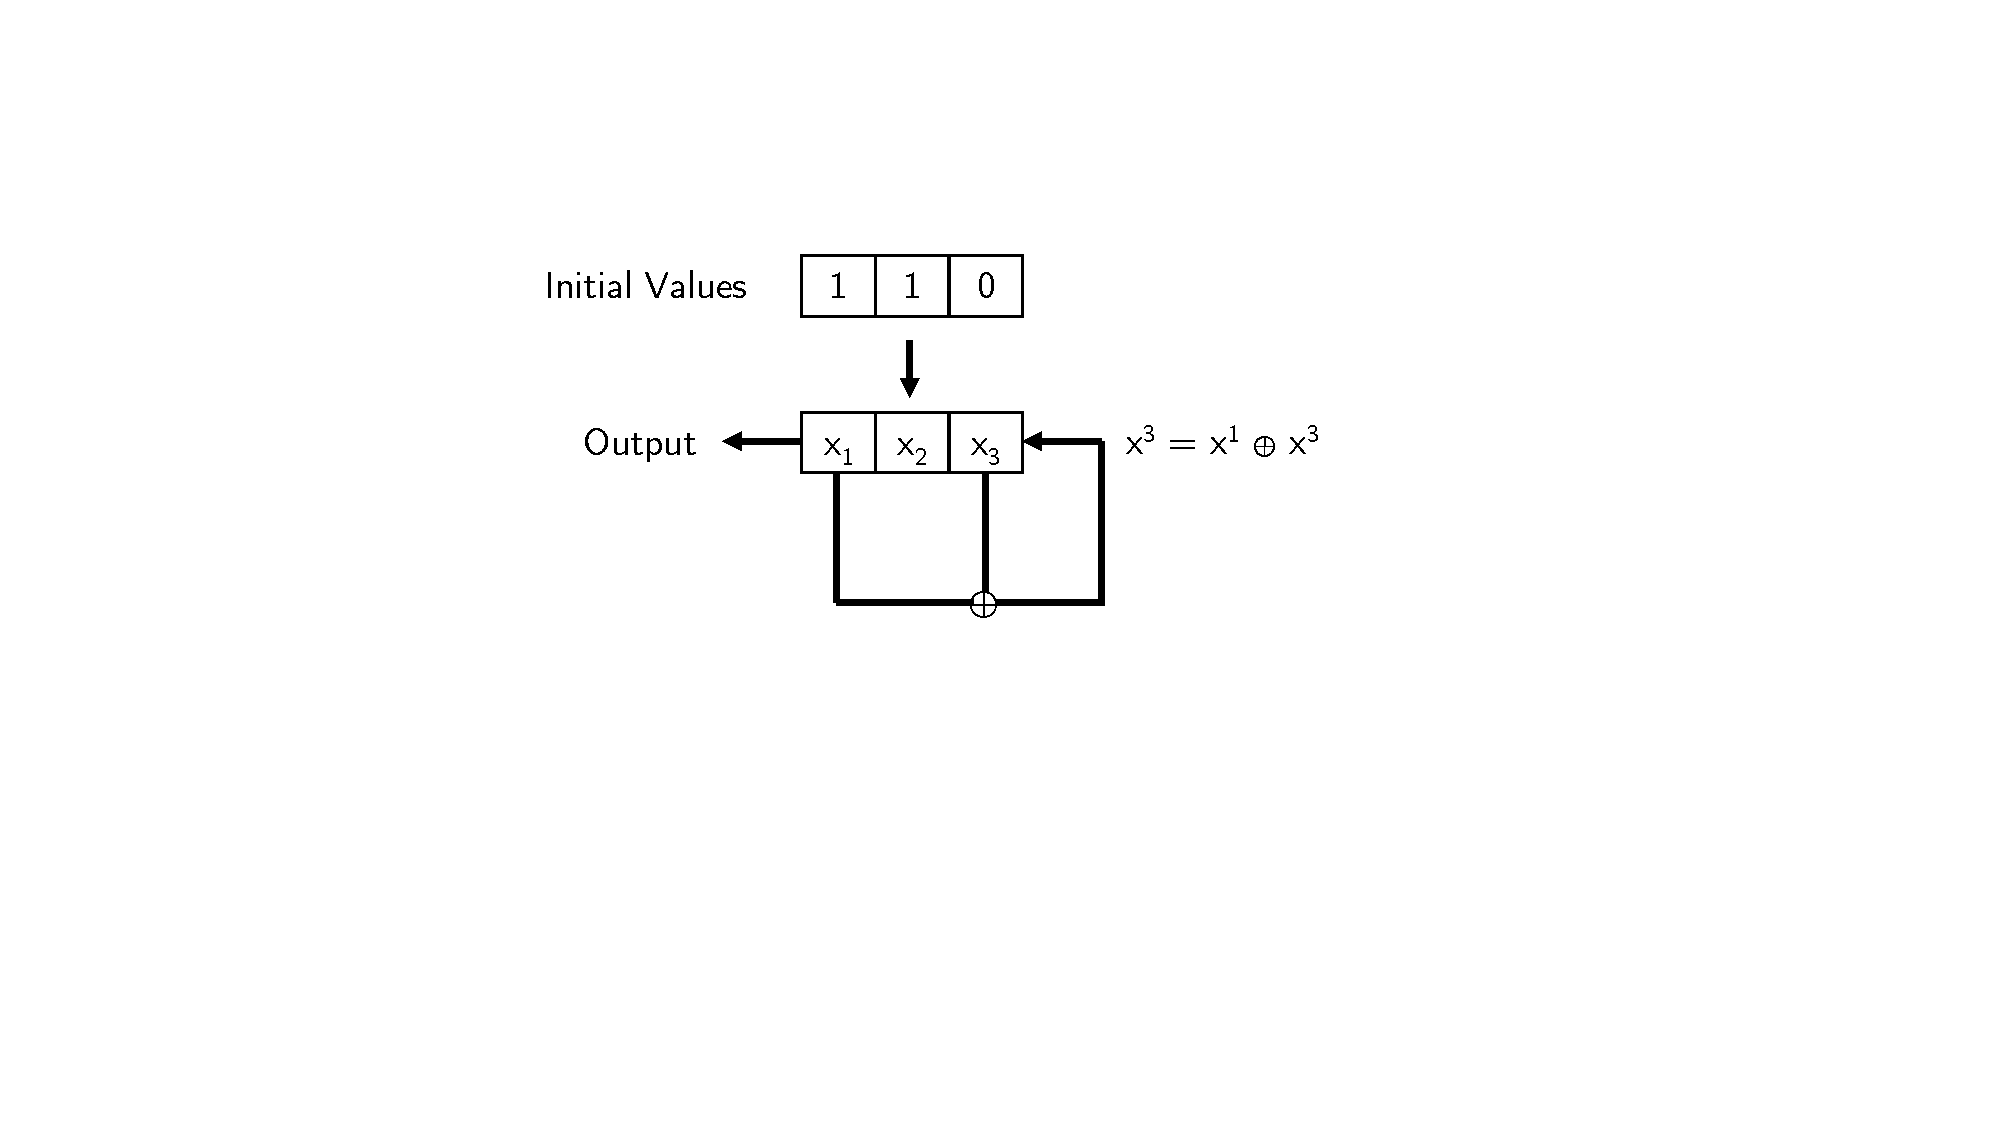
\includegraphics[width = \linewidth]{Linear Feedback Shift Register/Introduction.pdf}
		\caption{Given LFSR}
		\label{fig:lfsrintro}
	\end{subfigure}
	\begin{subfigure}[c]{0.45\linewidth}
		\centering
		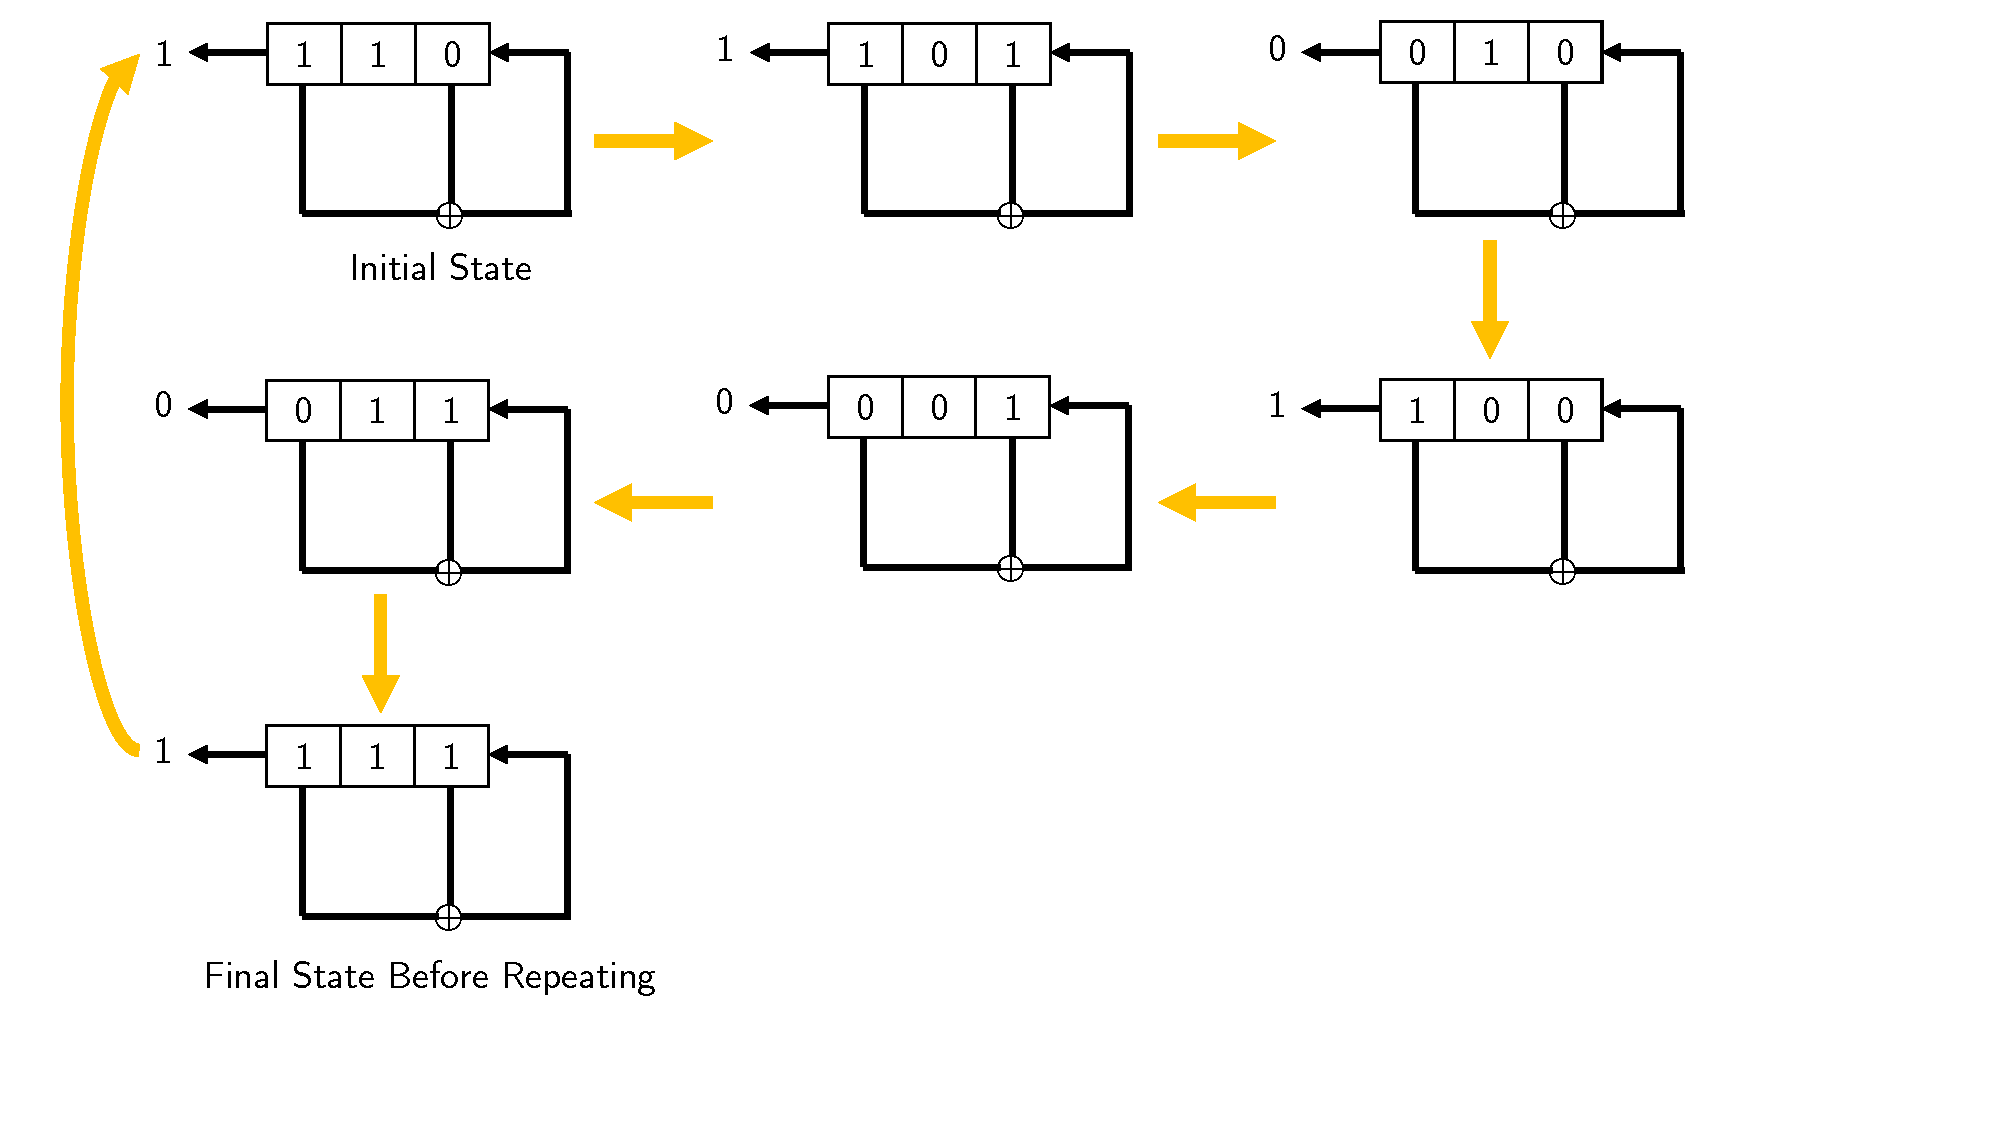
\includegraphics[width = \linewidth]{Linear Feedback Shift Register/Sequence Generation.pdf}
		\caption{The Generated Sequence is 11001001 repeating (follow the arrows)}
		\label{fig:lfsrgeneration}
	\end{subfigure}
	\caption{Linear Feedback Shift Register -- Working}
\end{figure}
\vspace{-2em}
\textbf{Problem Statement:}\\
A property of $n$ bit LFSR is that the output sequence it generates will start repeating in at most $2^{n-1}$ iterations called its period\footnote{Interestingly, there also exists a feedback polynomial which achieves this maximum period for every $n$.}.\\
Your task is to simulate an LFSR with a given initial state and feedback polynomial until it repeats and find its period\footnote{Is there a way to get the period of the sequence using just the feedback polynomial and without actually calculating sequence? The basis of this problem lie in the fascinating area of mathematics known as Abstract Algebra!
} in the process.
\begin{testcasesMore}
	{$t$ \hfill(number of test cases, an integer)\\
	$n_i\quad t_1\ t_2\ \cdots t_{n_i}\quad c_1\ c_2\ \cdots c_{n_i}$ \hfill($2n_i+1$ space seperated integers for each testcase)}
	{the output sequence generated by the given LFSR followed by the period of this output sequence\hfill(each iteration on a newline)}
	{$1 \leq n_i \leq 15$\\
	$t_i$ is either 0 or 1 and $c_1 = 1$\footnotemark,\ other $c_i$ are either 0 or 1\hfill(The LFSR will repeat from the beginning)}
	{1\quad 1 \quad 1\\2\quad1 0\quad1 0\\2 \quad 1 1 \quad 1 0\\2 \quad 1 1 \quad 1 1\\3 \quad 1 1 0 \quad 1 0 1\\5 \quad 1 0 1 0 0 \quad 1 0 0 1 0\\7 \quad 1 1 0 0 0 0 0 \quad 1 0 0 0 0 0 1}
	{1\quad1\\1 0\quad2\\1\quad1\\1 1 0\quad3\\1 1 0 1 0 0 1\quad7\\1 0 1 0 0 1 0 0 0 0 1 0 1 0 1 1 1 0 1 1 0 0 0 1 1 1 1 1 0 0 1\quad31\\1 1 0 0 0 0 0 1 0 0 0 0 0 0 1 1 1 1 1 1 1 0 1 0 1 0 1 0 0 1 1 0 0 1 1 1 0 1 1 1 0 1 0 0 1 0 1 1 0 0 0 1 1 0 1 1 1 1 0 1 1 0 1 0 1 1 0 1 1 0 0 1 0 0 1 0 0 0 1 1 1 0 0 0 0 1 0 1 1 1 1 1 0 0 1 0 1 0 1 1 1 0 0 1 1 0 1 0 0 0 1 0 0 1 1 1 1 0 0 0 1 0 1 0 0 0 0\quad127}
	{https://github.com/paramrathour/CS-101/tree/main/Test Cases/Linear Feedback Shift Register/Input.txt}
	{https://github.com/paramrathour/CS-101/tree/main/Test Cases/Linear Feedback Shift Register/Output.txt}
	{https://github.com/paramrathour/CS-101/tree/main/Starter Codes/Linear Feedback Shift Register.cpp}
\end{testcasesMore}
\footnotetext{This makes sure that the sequence will repeat from the beginning and will not have any non-periodic part. For example, $110101010\ldots$ (`10' repeating) is not possible if $c_1 = 1$.}
\begin{funvideo}
	\href{https://youtu.be/Ks1pw1X22y4}{Random Numbers with LFSR (Linear Feedback Shift Register) -- Computerphile}
\end{funvideo}
\KOMAoptions{paper=A4}
\recalctypearea